% one-figure manuscript written by fig_qc.py --tek-sekil-tex (trap T29)
\begin{figure}[!t]
\centering
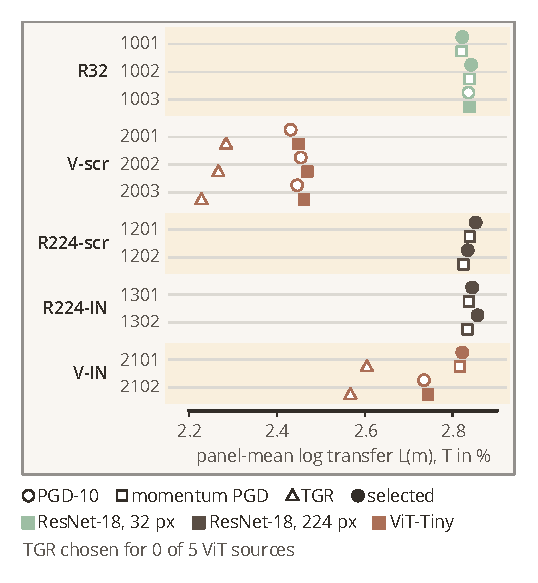
\includegraphics{fig10_attack_side}
\caption{\textbf{Transfer by attack, per source, on an abacus.} Each wire is one source; beads sit at its panel-mean log transfer L(m) under PGD-10 (circle), momentum PGD (square) and, for ViT sources, TGR (triangle). Filled beads are the attacks chosen by cross-fitted selection; TGR is never chosen. The value is the bead's position on the beam scale.}
\label{fig:fig10_attack_side}
\end{figure}
